\documentclass[11pt,openany]{article}

\input{algebra-note-preamble}
\input{tcolorbox}
\input{theorem}
\input{algebra-note-commands}
\usepackage{tikz}
\usepackage{tikz-cd}
\usepackage{tikz-3dplot}
\usepackage{amsmath}

\setstretch{1.25}
\begin{document}
\pagenumbering{arabic}
\begin{center}
	\huge\textbf{Quotient Rings, Closed Sets,\\ and Maximal Spectra}\\
	\vspace{0.5em}
	\large{Ji, Yong-hyeon}\\
	\vspace{0.5em}
	\normalsize{\today}\\
\end{center}
\[
\begin{tikzcd}[row sep=huge]
	\mathcal{A}
	\arrow[r, bend left=65, "F"{name=F}]
	\arrow[r, "G"{inner sep=0,fill=white,anchor=center,name=G}]
	\arrow[r, bend right=65, "H"{name=H, swap}]
	\arrow[from=F.south-|G,to=G,Rightarrow,shorten=2pt,"\alpha"] 
	\arrow[from=G,to=H.north-|G,Rightarrow,shorten=2pt,"\beta"] &
	\mathcal{B}.
\end{tikzcd} 
\]
\[
\begin{tikzcd}[row sep=huge]
	\mathscr{A} \arrow[r, "F"{sloped,above},"\hspace{0.15cm}\scalebox{1.5}{$\Downarrow$} \alpha"{sloped,below}, bend left=70] \arrow[r, "\hspace{0.15cm}\scalebox{1.5}{$\Downarrow$} \beta", "H"{sloped,below}, bend right=70] \arrow[r, "G" description] & \mathscr{B}
\end{tikzcd}
\]

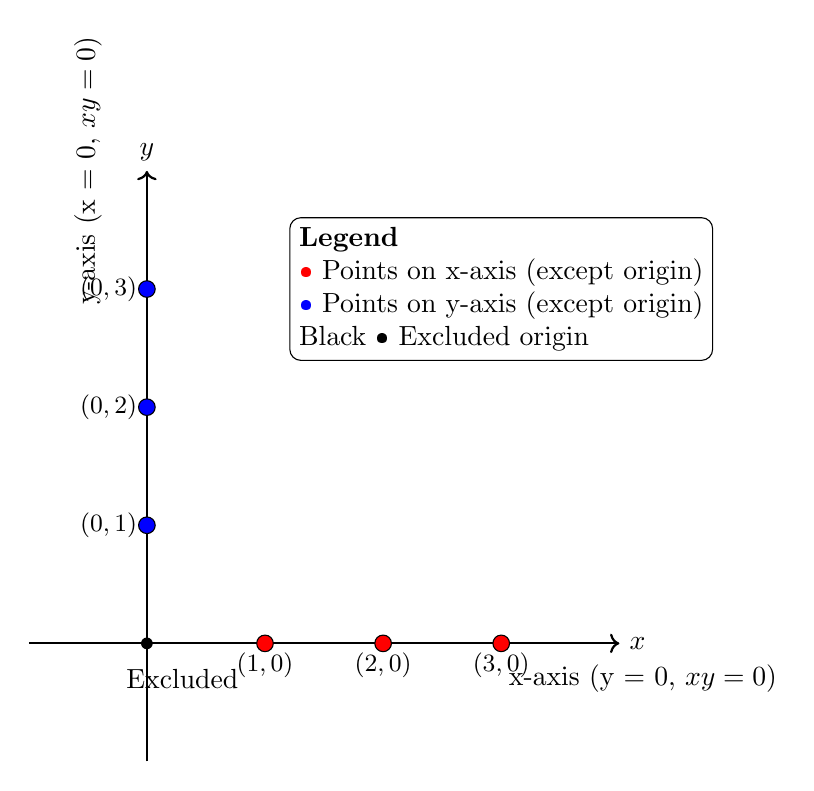
\begin{tikzpicture}[scale=1.5]
	% Axes
	\draw[thick, ->] (-1,0) -- (4,0) node[right] {$x$};
	\draw[thick, ->] (0,-1) -- (0,4) node[above] {$y$};
	
	% Axes labels
	\node at (4.2, -0.3) {x-axis (y = 0, \( xy = 0 \))};
	\node[rotate=90] at (-0.5, 4) {y-axis (x = 0, \( xy = 0 \))};
	
	% Points on the x-axis
	\foreach \x in {1, 2, 3}
	\draw[fill=red] (\x, 0) circle (2pt) node[below] {\small $(\x, 0)$};
	
	% Points on the y-axis
	\foreach \y in {1, 2, 3}
	\draw[fill=blue] (0, \y) circle (2pt) node[left] {\small $(0, \y)$};
	
	% Excluded origin point
	\node at (0,0) [circle, fill, inner sep=1.5pt]{};
	\node at (0.3, -0.3) {Excluded};
	
	% Legend
	\node[draw, fill=white, rounded corners, align=left] at (3, 3) {
		\textbf{Legend}\\
		\textcolor{red}{\textbullet} Points on x-axis (except origin)\\
		\textcolor{blue}{\textbullet} Points on y-axis (except origin)\\
		Black \textbullet{} Excluded origin
	};
\end{tikzpicture}

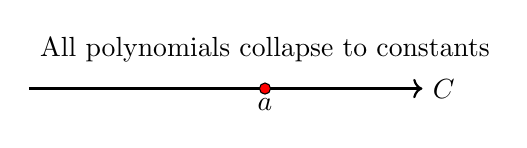
\begin{tikzpicture}
	% Axis
	\draw[thick, ->] (-1,0) -- (4,0) node[right] {$\mathbb{C}$};
	
	% Point at a
	\draw[fill=red] (2,0) circle (2pt) node[below] {$a$};
	
	% Label
	\node at (2, 0.5) {All polynomials collapse to constants};
\end{tikzpicture}

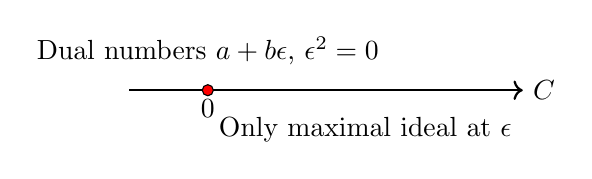
\begin{tikzpicture}
	% Axis
	\draw[thick, ->] (-1,0) -- (4,0) node[right] {$\mathbb{C}$};
	
	% Point at 0 (epsilon)
	\draw[fill=red] (0,0) circle (2pt) node[below] {$0$};
	
	% Label
	\node at (0, 0.5) {Dual numbers $a + b\epsilon$, $\epsilon^2 = 0$};
	\node at (2, -0.5) {Only maximal ideal at $\epsilon$};
\end{tikzpicture}

\begin{tikzpicture}
	% Axes
	\draw[thick, ->] (-3,0) -- (3,0) node[right] {$x$};
	\draw[thick, ->] (0,-1) -- (0,3) node[above] {$y$};
	
	% Points at x = b and x = -b
	\draw[fill=red] (2,0) circle (2pt) node[below right] {$b$};
	\draw[fill=red] (-2,0) circle (2pt) node[below left] {$-b$};
	
	% Labels
	\node at (0,-0.5) {$x^2 = a$ restricts $x$ to $\pm b$};
\end{tikzpicture}

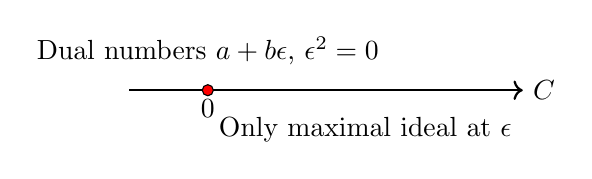
\begin{tikzpicture}
	% Axis
	\draw[thick, ->] (-1,0) -- (4,0) node[right] {$\mathbb{C}$};
	
	% Point at 0 (epsilon)
	\draw[fill=red] (0,0) circle (2pt) node[below] {$0$};
	
	% Label
	\node at (0, 0.5) {Dual numbers $a + b\epsilon$, $\epsilon^2 = 0$};
	\node at (2, -0.5) {Only maximal ideal at $\epsilon$};
\end{tikzpicture}

\section*{Example: \( R = \mathbb{C}[x, y] \) and \( I = \langle xy \rangle \)}

Let \( R = \mathbb{C}[x, y] \) and \( I = \langle xy \rangle \). Then the quotient ring \( R/I = \mathbb{C}[x, y]/\langle xy \rangle \) represents the ring of functions vanishing on the set \( V(I) \), which consists of points on the coordinate axes \( x = 0 \) and \( y = 0 \). The maximal ideals in \( R \) containing \( I \) correspond to points on these axes.

In this case:
\[
V(I) \cap \text{mSpec}(R) \cong \text{mSpec}(R/I)
\]
where \( V(I) \cap \text{mSpec}(R) \) includes all maximal ideals containing \( I \), which correspond to the points on the coordinate axes in \( \mathbb{C}^2 \).

\begin{center}
	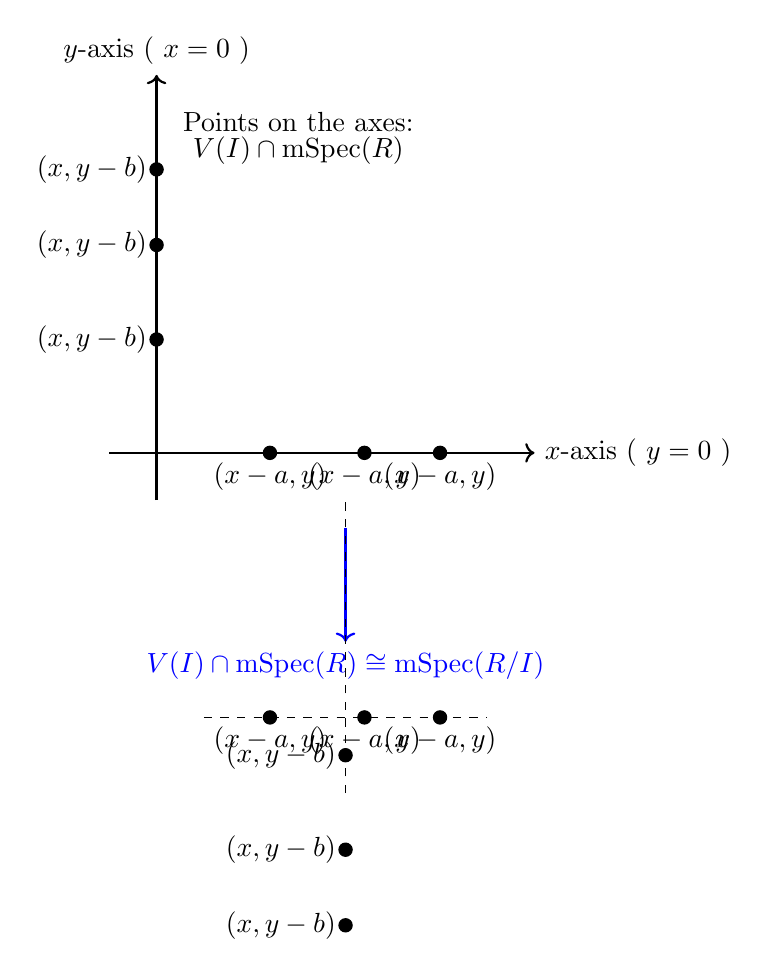
\begin{tikzpicture}[scale=1.2]
		
		% Draw coordinate axes
		\draw[thick, ->] (-0.5, 0) -- (4, 0) node[right] {\( x \)-axis ( \( y = 0 \) )};
		\draw[thick, ->] (0, -0.5) -- (0, 4) node[above] {\( y \)-axis ( \( x = 0 \) )};
		
		% Mark points on x-axis corresponding to maximal ideals (x - a, y)
		\foreach \a in {1.2, 2.2, 3} {
			\filldraw (\a, 0) circle (2pt);
			\node[anchor=north] at (\a, 0) {\( (x - a, y) \)};
		}
		
		% Mark points on y-axis corresponding to maximal ideals (x, y - b)
		\foreach \b in {1.2, 2.2, 3} {
			\filldraw (0, \b) circle (2pt);
			\node[anchor=east] at (0, \b) {\( (x, y - b) \)};
		}
		
		% Labels for V(I) intersection with mSpec(R)
		\node at (1.5, 3.5) {Points on the axes:};
		\node at (1.5, 3.2) {\( V(I) \cap \text{mSpec}(R) \)};
		
		% Correspondence arrow
		\draw[->, thick, blue] (2, -0.8) -- (2, -2);
		\node[below, blue] at (2, -2) {\( V(I) \cap \text{mSpec}(R) \cong \text{mSpec}(R/I) \)};
		
		% Draw the quotient ring mSpec(R/I) in lower part
		% Dashed lines representing axes in R/I
		\draw[dashed] (0.5, -2.8) -- (3.5, -2.8) node[right] {};
		\draw[dashed] (2, -3.6) -- (2, -0.5) node[above] {};
		
		% Points on axes in R/I
		\foreach \a in {1.2, 2.2, 3} {
			\filldraw (\a, -2.8) circle (2pt);
			\node[anchor=north] at (\a, -2.8) {\( (x - a, y) \)};
		}
		
		\foreach \b in {1.2, 2.2, 3} {
			\filldraw (2, -\b - 2) circle (2pt);
			\node[anchor=east] at (2, -\b - 2) {\( (x, y - b) \)};
		}
		
	\end{tikzpicture}
\end{center}

\section*{Explanation}

The points on the coordinate axes represent maximal ideals in \( R = \mathbb{C}[x, y] \) containing \( I = \langle xy \rangle \), which correspond to the points:
\begin{itemize}
	\item \( (x - a, y) \) for points on the \( x \)-axis (i.e., where \( y = 0 \) and \( x = a \)),
	\item \( (x, y - b) \) for points on the \( y \)-axis (i.e., where \( x = 0 \) and \( y = b \)).
\end{itemize}
Under the Zariski topology, this set \( V(I) \cap \text{mSpec}(R) \) is homeomorphic to \( \text{mSpec}(R/I) \), capturing the structure of the maximal spectrum in the quotient ring \( R/I \).


\newpage
\section*{1. Definition of a Homomorphism in Topology}

In topology, a \textbf{continuous map} or \textbf{homomorphism of topological spaces} is a function that preserves the structure of the topology. Formally:
\[
V(I) \cap \text{mSpec}(R) \cong \text{mSpec}(R/I),
\]
Let \( X \) and \( Y \) be topological spaces, with topologies \( \mathcal{T}_X \) and \( \mathcal{T}_Y \) respectively. A function \( f: X \to Y \) is called a \textbf{topological homomorphism} (or more commonly, a \textbf{continuous map}) if for every open set \( U \in \mathcal{T}_Y \), the preimage \( f^{-1}(U) \) is an open set in \( \mathcal{T}_X \). In other words:
\[
f \text{ is continuous if } \forall U \in \mathcal{T}_Y, \, f^{-1}(U) \in \mathcal{T}_X.
\]

This continuity condition ensures that the function \( f \) respects the topological structures of \( X \) and \( Y \).

\section*{2. Definition of the Zariski Topology}

The \textbf{Zariski topology} is a topology commonly used in algebraic geometry, particularly on the spectrum of a ring or on affine spaces. It is defined in terms of algebraic sets, which correspond to the vanishing of sets of polynomials.

\subsection*{On Affine Space}

Let \( \mathbb{A}^n = \mathbb{K}^n \) be the \( n \)-dimensional affine space over a field \( \mathbb{K} \). The Zariski topology on \( \mathbb{A}^n \) is defined by specifying that the closed sets are all \textbf{algebraic sets}. Specifically, a subset \( V \subseteq \mathbb{A}^n \) is closed if there exists a set of polynomials \( S \subseteq \mathbb{K}[x_1, \dots, x_n] \) such that:
\[
V = \{ \mathbf{a} \in \mathbb{A}^n : f(\mathbf{a}) = 0 \text{ for all } f \in S \}.
\]
The closed sets in this topology are precisely the sets of common zeros of families of polynomials, and the topology is coarser (i.e., has fewer open sets) than the standard topology on \( \mathbb{K}^n \) when \( \mathbb{K} \) is, for example, \( \mathbb{R} \) or \( \mathbb{C} \).

\subsection*{On the Spectrum of a Ring}

For a commutative ring \( R \), the \textbf{spectrum} \( \text{Spec}(R) \) is the set of all prime ideals of \( R \). The Zariski topology on \( \text{Spec}(R) \) is defined by taking the closed sets to be:
\[
V(I) = \{ \mathfrak{p} \in \text{Spec}(R) : I \subseteq \mathfrak{p} \},
\]
where \( I \) is an ideal of \( R \). In this context, \( V(I) \) is the set of all prime ideals containing \( I \), and these closed sets \( V(I) \) define the Zariski topology on \( \text{Spec}(R) \).

\section*{3. Definition of the Maximal Spectrum (\( \text{mSpec}(R) \))}

The \textbf{maximal spectrum} of a ring \( R \), denoted \( \text{mSpec}(R) \), is the set of all \textbf{maximal ideals} of \( R \).

Formally, \( \text{mSpec}(R) = \{ \mathfrak{m} \subset R : \mathfrak{m} \text{ is a maximal ideal of } R \} \).

When \( R \) is a commutative ring with identity, each maximal ideal \( \mathfrak{m} \in \text{mSpec}(R) \) corresponds to a "point" in an affine or projective variety over \( R \).

\subsection*{Topology on \( \text{mSpec}(R) \)}

The maximal spectrum \( \text{mSpec}(R) \) can be endowed with the \textbf{Zariski topology}, where the closed sets are defined as intersections of \( V(I) \) (closed sets in \( \text{Spec}(R) \)) with \( \text{mSpec}(R) \):
\[
V(I) \cap \text{mSpec}(R) = \{ \mathfrak{m} \in \text{mSpec}(R) : I \subseteq \mathfrak{m} \}.
\]
In other words, the closed sets in \( \text{mSpec}(R) \) are given by the maximal ideals containing a given ideal \( I \) of \( R \).

\newpage
To establish the relationship between quotient rings, closed sets, and maximal spectra, we are interested in the following formal statement and its proof.

\section*{Formal Statement}

Let \( R \) be a commutative ring, and let \( I \) be an ideal of \( R \). Then:
\begin{enumerate}
	\item There is a natural \textbf{homeomorphism} between \( V(I) \subseteq \text{Spec}(R) \), the set of prime ideals of \( R \) containing \( I \), and the \textbf{prime spectrum} \( \text{Spec}(R/I) \) of the quotient ring \( R/I \):
	\[
	V(I) \cong \text{Spec}(R/I).
	\]
	\item Similarly, there is a natural \textbf{homeomorphism} between \( V(I) \cap \text{mSpec}(R) \), the set of maximal ideals of \( R \) containing \( I \), and the \textbf{maximal spectrum} \( \text{mSpec}(R/I) \) of the quotient ring \( R/I \):
	\[
	V(I) \cap \text{mSpec}(R) \cong \text{mSpec}(R/I).
	\]
\end{enumerate}

\section*{Proof}

To prove this, we will demonstrate a natural correspondence between the prime ideals of \( R \) containing \( I \) and the prime ideals of \( R/I \), and we will show that this correspondence preserves the Zariski topology, making it a homeomorphism. Then we will restrict this correspondence to maximal ideals to establish the second part of the statement.

\subsection*{Part 1: Homeomorphism between \( V(I) \) and \( \text{Spec}(R/I) \)}

\textbf{Step 1: Define the Map from \( V(I) \) to \( \text{Spec}(R/I) \)}

Consider the \textbf{quotient map} \( \pi: R \to R/I \), defined by \( \pi(r) = r + I \). This map is surjective and induces a correspondence between certain ideals of \( R \) and ideals of \( R/I \):
\begin{itemize}
	\item For any prime ideal \( \mathfrak{p} \in \text{Spec}(R) \) that contains \( I \), the image \( \mathfrak{p}/I \subseteq R/I \) is a prime ideal in \( R/I \). Thus, for each \( \mathfrak{p} \in V(I) \), we obtain a prime ideal \( \mathfrak{p}/I \in \text{Spec}(R/I) \).
\end{itemize}

Define a map
\[
\phi: V(I) \to \text{Spec}(R/I)
\]
by
\[
\phi(\mathfrak{p}) = \mathfrak{p}/I.
\]

\textbf{Step 2: Show that \( \phi \) is Well-Defined and Surjective}

\begin{enumerate}
	\item \textbf{Well-Defined}: If \( \mathfrak{p} \in V(I) \), then \( I \subseteq \mathfrak{p} \), and \( \mathfrak{p}/I \) is a prime ideal in \( R/I \). Thus, \( \phi(\mathfrak{p}) = \mathfrak{p}/I \in \text{Spec}(R/I) \).
	
	\item \textbf{Surjectivity}: For any prime ideal \( \mathfrak{q} \in \text{Spec}(R/I) \), consider the preimage of \( \mathfrak{q} \) under \( \pi \):
	\[
	\psi(\mathfrak{q}) = \pi^{-1}(\mathfrak{q}) = \{ r \in R : r + I \in \mathfrak{q} \}.
	\]
	This set \( \psi(\mathfrak{q}) \) is a prime ideal in \( R \) that contains \( I \), so \( \psi(\mathfrak{q}) \in V(I) \) and \( \phi(\psi(\mathfrak{q})) = \mathfrak{q} \). Therefore, \( \phi \) is surjective.
\end{enumerate}

\textbf{Step 3: Define the Inverse Map}

We define the inverse map \( \psi: \text{Spec}(R/I) \to V(I) \) by
\[
\psi(\mathfrak{q}) = \pi^{-1}(\mathfrak{q}).
\]
This map takes each prime ideal \( \mathfrak{q} \in \text{Spec}(R/I) \) to a prime ideal in \( R \) containing \( I \).

\begin{itemize}
	\item \textbf{Well-Defined}: Since \( \mathfrak{q} \) is a prime ideal in \( R/I \), its preimage \( \psi(\mathfrak{q}) = \pi^{-1}(\mathfrak{q}) \) is a prime ideal in \( R \) containing \( I \).
	\item \textbf{Inverse Property}: For \( \mathfrak{p} \in V(I) \), we have \( \psi(\phi(\mathfrak{p})) = \psi(\mathfrak{p}/I) = \mathfrak{p} \), and for \( \mathfrak{q} \in \text{Spec}(R/I) \), we have \( \phi(\psi(\mathfrak{q})) = \phi(\pi^{-1}(\mathfrak{q})) = \mathfrak{q} \).
\end{itemize}

Thus, \( \phi \) and \( \psi \) are inverse maps, establishing a bijection between \( V(I) \) and \( \text{Spec}(R/I) \).

\textbf{Step 4: Show that \( \phi \) is a Homeomorphism}

To prove that \( \phi \) is a homeomorphism, we need to show that it preserves the \textbf{Zariski topology}.

\begin{itemize}
	\item \textbf{Closed Sets in \( V(I) \)}: In \( \text{Spec}(R) \), a closed set is of the form \( V(J) = \{ \mathfrak{p} \in \text{Spec}(R) : J \subseteq \mathfrak{p} \} \) for some ideal \( J \subseteq R \). The closed sets in \( V(I) \) are intersections of closed sets in \( \text{Spec}(R) \) with \( V(I) \), so they are of the form \( V(J) \cap V(I) \) for some \( J \subseteq R \).
	
	\item \textbf{Corresponding Closed Sets in \( \text{Spec}(R/I) \)}: Closed sets in \( \text{Spec}(R/I) \) are of the form \( V(J') = \{ \mathfrak{q} \in \text{Spec}(R/I) : J' \subseteq \mathfrak{q} \} \) for some ideal \( J' \subseteq R/I \).
\end{itemize}

The map \( \phi \) takes \( V(J) \cap V(I) \) in \( \text{Spec}(R) \) to \( V(J/I) \) in \( \text{Spec}(R/I) \), preserving the closed sets and making \( \phi \) a homeomorphism.

Thus, we have shown:
\[
V(I) \cong \text{Spec}(R/I).
\]

\subsection*{Part 2: Homeomorphism between \( V(I) \cap \text{mSpec}(R) \) and \( \text{mSpec}(R/I) \)}

The same argument holds when we restrict to maximal ideals. Since \( \phi \) and \( \psi \) preserve inclusion, they also induce a bijection between maximal ideals containing \( I \) and maximal ideals in \( R/I \).

\begin{itemize}
	\item A maximal ideal \( \mathfrak{m} \in \text{mSpec}(R) \) containing \( I \) maps to a maximal ideal \( \mathfrak{m}/I \in R/I \).
	\item Conversely, any maximal ideal \( \mathfrak{m}' \in \text{mSpec}(R/I) \) has a preimage under \( \pi \) that is a maximal ideal containing \( I \).
\end{itemize}

Thus, we have a bijection:
\[
V(I) \cap \text{mSpec}(R) \cong \text{mSpec}(R/I),
\]
and this bijection preserves the Zariski topology, making it a homeomorphism.

\section*{Conclusion}

We have shown that:
\begin{enumerate}
	\item \( V(I) \cong \text{Spec}(R/I) \) as topological spaces in the Zariski topology.
	\item \( V(I) \cap \text{mSpec}(R) \cong \text{mSpec}(R/I) \), also as topological spaces.
\end{enumerate}

This establishes the relationship between the quotient ring \( R/I \), the closed set \( V(I) \), and the maximal spectra.

\newpage
\section*{Introduction}

In commutative algebra and algebraic geometry, the process of **localization** at a prime ideal \( \mathfrak{p} \) in a ring \( R \) allows us to focus on the behavior of \( R \) near \( \mathfrak{p} \). This process induces a natural continuous map on spectra in the **Zariski topology**. Here, we describe this topological homomorphism in detail.

\section*{Definition of Localization and the Induced Map}

Let \( R \) be a commutative ring, and let \( \mathfrak{p} \) be a prime ideal in \( R \). Define \( S = R \setminus \mathfrak{p} \), a multiplicatively closed set of elements in \( R \) that are not in \( \mathfrak{p} \). The **localization of \( R \) at \( \mathfrak{p} \)**, denoted \( R_{\mathfrak{p}} \), is the ring where elements of \( S \) are inverted:
\[
R_{\mathfrak{p}} = S^{-1} R = \left\{ \frac{a}{s} : a \in R, s \in S \right\}.
\]
The localization \( R_{\mathfrak{p}} \) effectively "focuses" on the structure of \( R \) around the prime ideal \( \mathfrak{p} \).

\textbf{Topological Homomorphism on Spectra}

Localization induces a continuous map on the prime spectra in the Zariski topology:
\[
f: \text{Spec}(R_{\mathfrak{p}}) \to \text{Spec}(R),
\]
where each prime ideal \( \mathfrak{q} \in \text{Spec}(R_{\mathfrak{p}}) \) maps to a prime ideal \( f(\mathfrak{q}) = \mathfrak{q} \cap R \) in \( R \).

\subsection*{Definition of the Map \( f \)}

1. **Mapping**: Define \( f: \text{Spec}(R_{\mathfrak{p}}) \to \text{Spec}(R) \) by
\[
f(\mathfrak{q}) = \mathfrak{q} \cap R.
\]
This map takes a prime ideal \( \mathfrak{q} \) in \( R_{\mathfrak{p}} \) and restricts it to \( R \) by intersecting it with \( R \). Since the preimage of a prime ideal under a localization map is prime, \( f(\mathfrak{q}) \) is a prime ideal in \( R \).

2. **Image of the Map**: The image of \( f \) is the set of prime ideals in \( R \) that are contained within \( \mathfrak{p} \):
\[
\text{Im}(f) = \{ \mathfrak{p}' \in \text{Spec}(R) : \mathfrak{p}' \subseteq \mathfrak{p} \}.
\]
This corresponds to the closed set \( V(\mathfrak{p}) \subseteq \text{Spec}(R) \) in the Zariski topology.

3. **Continuity of \( f \)**: The map \( f \) is continuous with respect to the Zariski topology. Recall that in the Zariski topology, a closed set in \( \text{Spec}(R) \) is defined by \( V(I) = \{ \mathfrak{p}' \in \text{Spec}(R) : I \subseteq \mathfrak{p}' \} \) for an ideal \( I \subseteq R \). The preimage of a closed set \( V(I) \) in \( \text{Spec}(R) \) under \( f \) is the closed set \( V(I R_{\mathfrak{p}}) \) in \( \text{Spec}(R_{\mathfrak{p}}) \), ensuring that \( f \) preserves the closed sets.

\section*{Interpretation in Algebraic Geometry}

In algebraic geometry, the map \( f: \text{Spec}(R_{\mathfrak{p}}) \to V(\mathfrak{p}) \subseteq \text{Spec}(R) \) corresponds to **localizing at the point** associated with \( \mathfrak{p} \). This allows us to study the local properties of varieties, such as local rings and germs of functions at a point, which are fundamental in understanding the structure of varieties and schemes.


\end{document}
